\documentclass[12pt,a4paper,oneside,english]{book}

\usepackage{cite}


%\usepackage[latin1]{inputenc}

%\usepackage[T1]{fontenc}
\usepackage[english]{babel}
\usepackage{amsmath}
\usepackage{amsfonts}
\usepackage{amssymb}
\usepackage{graphicx}
\usepackage{subfig}
\usepackage{fancyhdr}
\usepackage{appendix}
\usepackage{hyphenat}
\usepackage{pdfpages}
\usepackage{svg}

%\usepackage{tocloft} % For TOC customization ( table of contents )
\usepackage{array,multirow,makecell}
\newcolumntype{C}[1]{>{\arraybackslash}p{#1}}

\usepackage{enumitem}
\setlist{leftmargin=*,itemsep=0pt}

\usepackage{centernot}
\usepackage[linesnumbered,ruled,vlined,english,onelanguage]{algorithm2e}

\usepackage{quotchap}
\makeatletter
\renewcommand{\@makechapterhead}[1]{
 \chapterheadstartvskip
 {\size@chapter{\sectfont\raggedright
 {\chapnumfont
 \ifnum \c@secnumdepth >\m@ne
 \if@mainmatter\thechapter %frontmatter for roman numerals
 \fi\fi
 \par\nobreak}
 {\raggedright\advance\leftmargin10em\interlinepenalty\@M #1\par}}
 \nobreak\chapterheadendvskip}}
\makeatother
\renewcommand*{\chapterheadendvskip}{\vspace{2cm}}
%\renewcommand{\thechapter}{\Roman{chapter}} % Set chapter numbering to Roman numerals


\usepackage{geometry}
\geometry{hmargin=2cm,vmargin=2cm}

\pagestyle{fancyplain}
\lhead{\fancyplain{}{\nouppercase{\textit{\leftmark}}}}
\chead{\fancyplain{}{}}
\rhead{\fancyplain{}{}}
\lfoot{\fancyplain{}{}}
\cfoot{\fancyplain{}{}}
\rfoot{\fancyplain{\thepage}{\thepage}}
\renewcommand{\headrulewidth}{1pt}
\renewcommand{\footrulewidth}{1pt}

\renewcommand{\thesection}{\Roman{section}} % Set section numbering to Roman numerals % previously \arabic{section}

\usepackage{titlesec}
\titleformat{\paragraph}{\fontsize{11}{10}\bfseries}{\theparagraph}{1em}{}
\titlespacing*{\paragraph}{0pt}{10pt plus 2pt minus 0pt}{0pt plus 2pt minus 0pt}

\setcounter{secnumdepth}{4}
\setcounter{tocdepth}{4}

\usepackage{array}
\usepackage{multirow}
%\addto\captionsfrench{\def\tablename{\textsc{Tableau}}}

%\DefineBibliographyStrings{french}{urlseen = {},}

\setlength{\parskip}{0pt}%was 8 : space between paragraphs
\setlength{\parindent}{1.5em}%was 1.5 : indentation of paragraphs

\usepackage{setspace}

\usepackage{url}

\usepackage{hyperref}
% Comment before printing to remove links' colors
\definecolor{darkblue}{rgb}{0.0, 0.0, 0.5}
\hypersetup{
 colorlinks,
 linktocpage=true,
 linkcolor={darkblue},
 citecolor={darkblue},
 urlcolor={blue}}

\sloppy

\author{You}
\title{Internship Report}

\begin{document}
\pagenumbering{gobble}
\includepdf[pages=-]{FrontPage.pdf}
\chapter*{Acknowledgments}

\frontmatter %here yothhrou les num des pages en bas 
\chapter*{Abstract}
\normalsize{Write your abstract here.

\medskip
{\noindent \textbf{Keywords: ..., ... .} }

\spacing{1}
\tableofcontents{}
\newpage 
\listoffigures
\newpage 
\listoftables
\newpage
\spacing{1.4}
\chapter*{List of acronyms}
%\addcontentsline{toc}{chapter}{Liste des acronymes}
\markboth{List of acronyms}{}%abbrev
\begin{itemize}
\item \textbf{AI} Artificial Intelligence
\item \textbf{ML} Machine Learning
\item \textbf{API} Application Programming Interface
\item \textbf{ASR} Automatic Speech Recognition
\item \textbf{SER} Speech Emotion Recognition
\item  \textbf{NLP} Natural Language Processing
\item \textbf{DBSCAN} Density-Based Spatial Clustering of Applications with Noise
\item \textbf{GIS} Geographical Information System
\item \textbf{GPS} Global Positioning System

\end{itemize}

\frontmatter %here yothhrou les num des pages fl contnent
%\frontmatter  %to have roman page numbering in the beginning
%\mtcaddchapter[Introduction g�n�rale]

\chapter*{Introduction}
\addcontentsline{toc}{chapter}{Introduction}
\markboth{Introduction}{}

\chapter{Company Presentation} % we should metion that there are a lot of spacing between title of chapter and sctions

\label{ch:1er}
\section{Overview}
Founded in 2020, and located in both Meudon la forêt , Meudonn France and tunis, Tunisia, 
Hydatis is dedicated to helping early-stage companies leverage the latest data intelligence and digital technologies to solve real-world challenges, becoming, since then, a leading technology startup studio with a proven track record.
\begin{figure}[h!] % placement options: h=here, t=top, b=bottom, p=page
    \centering
    
\includegraphics[width=0.2\textwidth]{images/hydatiss.png}
    \caption{Logo of Hydatis}
    \label{fig:hydatis}
\end{figure}

Hydatis specializes in AI, machine learning, blockchain, big data Analysis and more. Hydatis's team of technology experts is dedicated to building scalable and sustainable businesses, with a focus on creativity, strategy, and technology alongside with a vast network of partners and investors and a strong reputation in the technology industry.
\begin{figure}[h!] % placement options: h=here, t=top, b=bottom, p=page
    \centering
    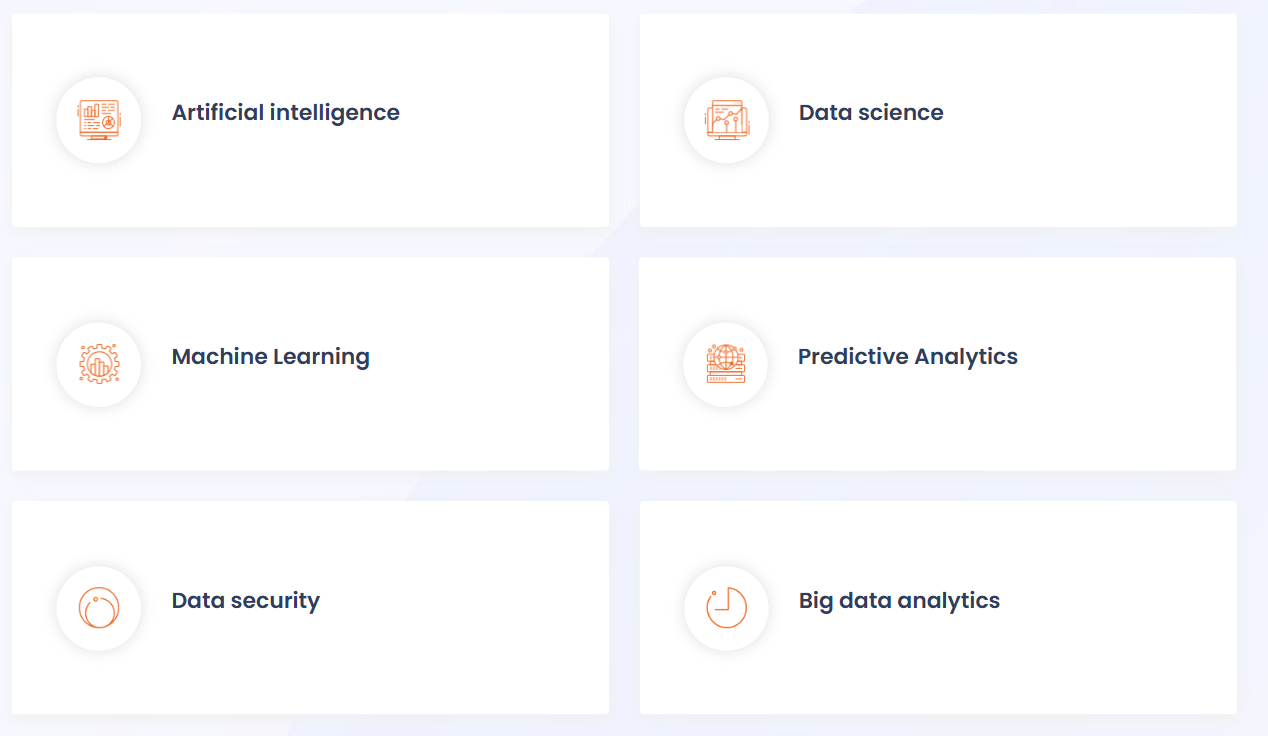
\includegraphics[width=0.699\textwidth]{images/Expertise_hydatis.png}
    \caption{Hydatis' Areas of Expertise}
    \label{fig:Expertise_hydatis}
\end{figure}

\section{Sectors of Activities}%and services offered
Hydatis is a product-focused Tech venture studio offering a range of services tailored to the unique needs of each startup, including:
 business planning, product development, marketing, and fundraising. 
%With their expertise in data analytics, machine learning, and other advanced technologies, 
Leveraging technology and entrepreneurship, they help clients turn data into actionable insights that drive business success.
%help businesses make big decisions about their future by making tangible versions of tomorrow.
\subsection{Services offered}
\begin{itemize}
    \item \textbf {Software development Services}
    \item \textbf{CTO as a service}
    \item \textbf{IT Consulting}
    \item \textbf{Devops Consulting}
    \item \textbf{and a lot more...}
\end{itemize}
\begin{figure}[h!]
    \centering
    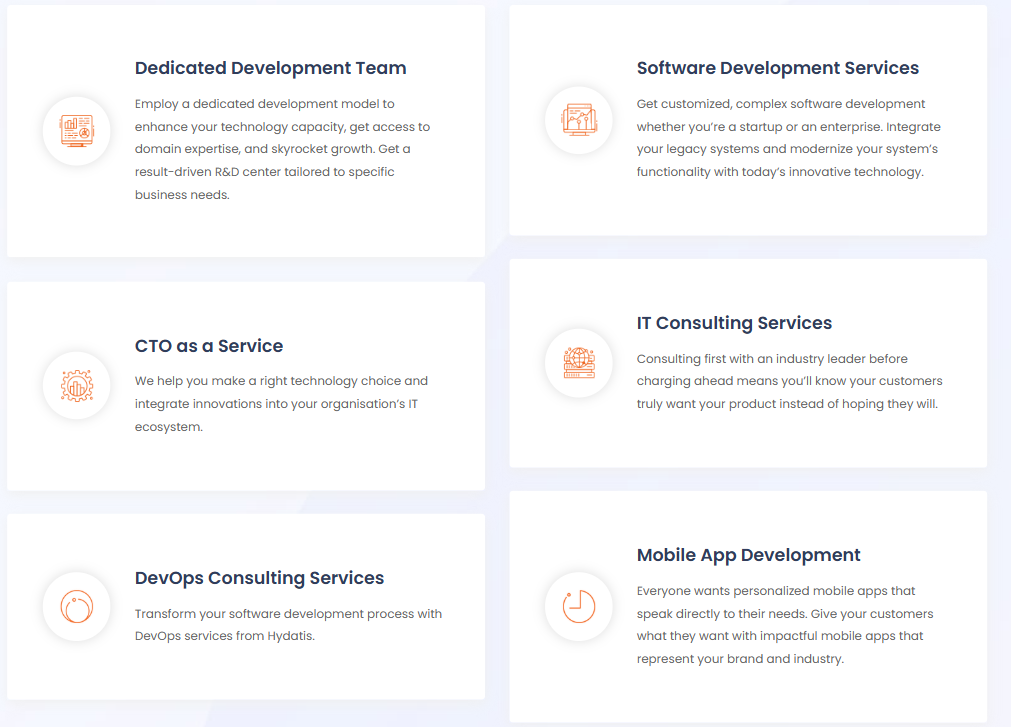
\includegraphics[width=0.9\textwidth]{images/services_hydatis.png}
    \caption{Hydatis' Services}
    \label{fig:Services_hydatis}
\end{figure}

\section{Organizational structure and Human Capital} % eithr this part will be deleted or the susection in the activities section will be modified and either discard items or having an individual subsection
Hydatis with a flat organizational structure that reflects its startup studio roots, led by  expertised directors who drive strategy and innovation alongside a talented crew of entrepreneurs and technologists, business strategists and network coordinators.

From AI specialists shaping cutting-edge products to strategists securing partnerships, and sicne its launch in 2020, these folks, with their varied backgrounds, suceeded to make Hydatis a powerhouse in the startup ecosystem.


\chapter{Internship Context and Objectives}
\label{ch:2eme}
\section{Problem Statement and Motivation} %Why
Crime is a major social problem in Tunisia, threatening public safety and disrupting the economy,ranging from theft to harassment, often leaving individuals vulnerable, especially at night or in isolated spots.
 
Traditional safety solutions such as manual reporting or basic wearable alarms have served as a foundational step in personal security. However they %struggle
suffer from critical limitations: 
The binary nature of a simple button press is usually unsufficient to distinguish between 
a genuine, life-threatening emergency,a false alarm, or a low-priority situation.
Additionally, the lack of contextual awarness results in inaccurate alerts and overwhelming emergency services with false positives. %Inaccuracy and Context Deficiency:
Giving the limited resources of emergency services (police, paramedics), false alarms divert critical attention away from genuine crises, incurring unnecessary costs and potentially delaying responses to real incidents. %Resource Depletion:


%The binary nature of a simple button press: unsufficient to distinguish between 
%a genuine, life-threatening emergency,a false alarm, or a low-priority situation. This leads to an unacceptably 
%high rate of false positives.

%  This gap hits home for Hydatis, the motivation behind this work is clear: we need to move beyond simple, reactive triggers
% and build smarter, faster ways to protect people by qualifying alerts with precision.
\subsection{Market Context and Existing Solutions}

Several commercial solutions exist in the personal safety market, including panic button apps like 
bSafe, location-sharing platforms like Life360, and wearable devices such as personal alarms. However,
 these solutions typically operate independently and lack the intelligent analysis needed to 
 differentiate between genuine emergencies and false alarms and ensure fast response to threats. 
 %, leading to the limitations described above.
Therefore, there is a clear need for an intelligent safety system that can analyze multiple data 
streams—location, audio, and behavioral patterns—to provide accurate, context-aware emergency 
detection while minimizing false positives.

%In State of the Art, you can include:
%Existing products (apps, devices, services → e.g., SOS apps, smartwatches with panic buttons, crime reporting platforms).
%Research/technical approaches (papers on anomaly detection, crime prediction models, wearable safety devices).
%Limitations of these (false positives, lack of contextual awareness, poor adoption, battery issues, limited reach, etc.).

%Detailed technical comparisons
%Algorithm discussions
%Academic literature reviews
%In-depth analysis of existing methods

%todo: reduce space in the footer ( especially see this page!)
%todo: and fama paget fihom khatt fl footer o whayed lee

\section{Description}% or scope : the "What." and "how" A high-level overview of the solution.

This project involves designing an AI-powered module for a Smart wearable Solution, aimed at enhancing personal safety through automated incident detection during my Summer internship at Hydatis.
The module integrates four key data streams: 
\begin{itemize}
    \item \textbf{Geospatial Analysis:} geospatial data derived from Tunisian crime datasets to identify high-risk areas.
    \item \textbf{Vocal Signal Processing:}  real-time vocal analysis to detect distress signals or key words such as calls for help.
    \item \textbf{Behavioral Profiling:} behavioral patterns to flag anomalies in user activitythat may indicate danger.
    \item \textbf{Decision Engine:} later, these components are fused into a cohesive system that processes and combines 
insights from each stream, offering a foundation for reliable alert qualification.
\end{itemize}
Though, detailed implementation will be explored in later sections.


\section{Core Mission, Objectives and Expected Results}

\subsection{Core Mission}
My core mission in this project is to develop an intelligent, multi-modal safety system that integrates  geospatial analysis, vocal processing, and behavioral profiling to transform personal security and  provide accurate , context-aware emergency detection that minimizes false alarms while ensuring genuine immediate attention to genuine threats  .

\subsection{Main Objectives}

\textbf{Technical Objectives:}
\begin{itemize}
    \item Achieve a minimum of 80\% accuracy in alert qualification.
    \item Minimize false positive rates. 
    \item Enable real-time processing  with response times under 5 seconds.
    \item Design a robust system capable of handling diverse scenarios and user behaviors.
\end{itemize}

\textbf{Implementation Objectives:}
\begin{itemize}

\item Process a Tunisian crime dataset for geospatial risk assessment.
\item Train a vocal ASR model adapted to Tunisian dialects for distress-related risk detection.
\item Prepare a vocal pipeline to analyse vocal patterns including: tone, rythm, and pitch.
\item Design a comprehensive database of processed behavioral patterns for every user.
   \item Integrate three distinct AI modules (geospatial, vocal, behavioral) into a cohesive system.
    \item Develop a proof-of-concept API for periodic risk assessment and scoring alerts.
    \item Ensure system scalability for potential deployment beyond Tunisia.
\end{itemize}

\subsection{Expected Results}
\begin{itemize}
\item A cleaned and structured Tunisian crime dataset inferred to geospatial risk analysis.
\item An ASR model integrated for vocal analysis in tunisian Arabic. %supporting real-time distress detection.
\item A vocal pipeline capable of analysing vocal patterns of stress and/or fear.
\item ML models designed for inferring  users behaviors.
\item A proof-of-concept multi-modal scoring system with sub-5-second responses.
\item APIs developed for periodic risk assessment and potential integration into a mobile or web interface.
\end{itemize}


\section{Internship timeline }% or planning %professionalism and project management skills.%%%%%often a Gantt chart)
%Timeline = just dates and deadlines
%Planning = timeline + methodology + resources + milestones

This project is structured over my two-month internship period at Hydatis, devided into:
\begin{itemize}
    \item \textbf{Weeks 1-2:} Initial research, dataset acquisition, and preprocessing.
    \item \textbf{Weeks 3-4:} Development of the geospatial analysis module and initial vocal processing pipeline.
    \item \textbf{Weeks 5-6:} Behavioral profiling model development and integration of the three AI modules.
    \item \textbf{Weeks 7-8:} Final system integration, testing, optimization, and documentation.
\end{itemize}

%todo: label the sections and subsections
%todo: diagramme de gantt!!!!

\chapter{Theoritical Foundations and State of the Art}
\label{ch:3eme}

% normalement we should put here:  State of the Art and Market Solutions section
% or subsection in the motivation and problem statement section: Existing Solutions and Limitations”
\section*{Introdunction}
This chapter presents the theoretical foundations underlying the proposed multi-modal safety system, which integrates three distinct yet complementary technologies:

First, the principles of geospatial analysis for risk prediction will be examined. 
Second, the field of vocal signal processing for distress detection will be explored, detailing the methods used to identify audible signs of an emergency from a user's speech. 
Finally, the concepts of machine learning applied on behavioral anomaly detection will be discussed, explaining the detection of anomalies based on personal routines.
\\This review justifies the technical choices made in the subsequent implementation chapter.
%establishes the scientific basis for
\section{Geospatical Analysis for Risk Prediction}
\label{sec:geospatial_theory}

Geospatial analysis integrates Geographical Information Systems (GIS) with advanced analytical techniques to identify crime hotspots, cluster incidents, and enable real-time risk assessment. This section explores hotspot forecasting, density-based clustering, and the evolution toward real-time systems, aligning with the need for intelligent personal safety solutions.

%This section establishes the theoretical foundations for location-based risk assessment module, which forms a core component 
%of the proposed multi-modal safety system.
%The analysis begins with crime hotspot theory and spatial clustering principles. Subsequently, density-based clustering algorithms, 
%particularly DBSCAN, are examined. Finally, the transition from static crime mapping to real-time risk assessment systems is explored.


\subsection{Crime Hotspot Forecasting and Spatial Analysis}


%Geospatial anomaly detection leverages Geographical Information Systems (GIS) to identify unusual patterns in spatial data, 
%a critical step in predicting crime hotspots. GIS integrates spatial datasets—such as crime locations, demographic details, 
%and environmental factors—into a unified framework for analysis [El-Fishawy et al., 2024]. 
%W ANTED TO PUT IT HERE

The foundational principle of crime hotspot analysis is that criminal activity is not randomly 
distributed, but rather concentrated in specific areas known as 'hotspots'
This involves analyzing geographic patterns where crime incidents cluster,
often influenced by factors like urban density or offender homogeneity \cite{chen2019exploring}. 
Hotspot theory posits that such clusters represent areas of elevated risk, necessitating targeted interventions  \cite{zhuang2017crime} .
With the ever-increasing ability of states and organizations to collect and store detailed data tracking crime occurrence, a significant amount of data with spatial and temporal information has been collected
In this context, these hotspots, defined as deviations from expected spatial-temporal behavior, can be treated as a form of spatial anomaly and can be detected using statistical and machine learning techniques, enabling the identification of high-risk areas.

\subsection{Density-Based Clustering for Spatial Data}%or for geographic data
\label{sec:dbscan_theory}
Crime data is inherently noisy and unevenly distributed, making it challenging to identify meaningful patterns using simple statistical methods. Clustering techniques are therefore employed to detect areas 
where incidents concentrate, which often correspond to crime hotspots.
%Spatial clustering is a process of grouping objects based on their spatial similarity. 

Among the available clustering algorithms, density-based methods such as DBSCAN \textbf{(Density-Based Spatial Clustering of Applications with Noise) } \cite{BIRANT2007208dbscan} are particularly effective for spatial data, a method well-suited for irregular,
 non-spherical patterns.
 \\
DBSCAN groups data points that are closely packed together and marks outliers as noise based on their density in the feature space.
Unlike other methods of clustering such as K-Means, it performs well in handling real-world data irregularities such as:
\begin{itemize}
    \item Arbitrary-Shaped Clusters: Clusters can take any shape not just circular or convex.
    \item Noise and Outliers: It effectively identifies and handles noise points without assigning them to any cluster.
\end{itemize}

\begin{figure}[h!] % placement options: h=here, t=top, b=bottom, p=page
    \centering
    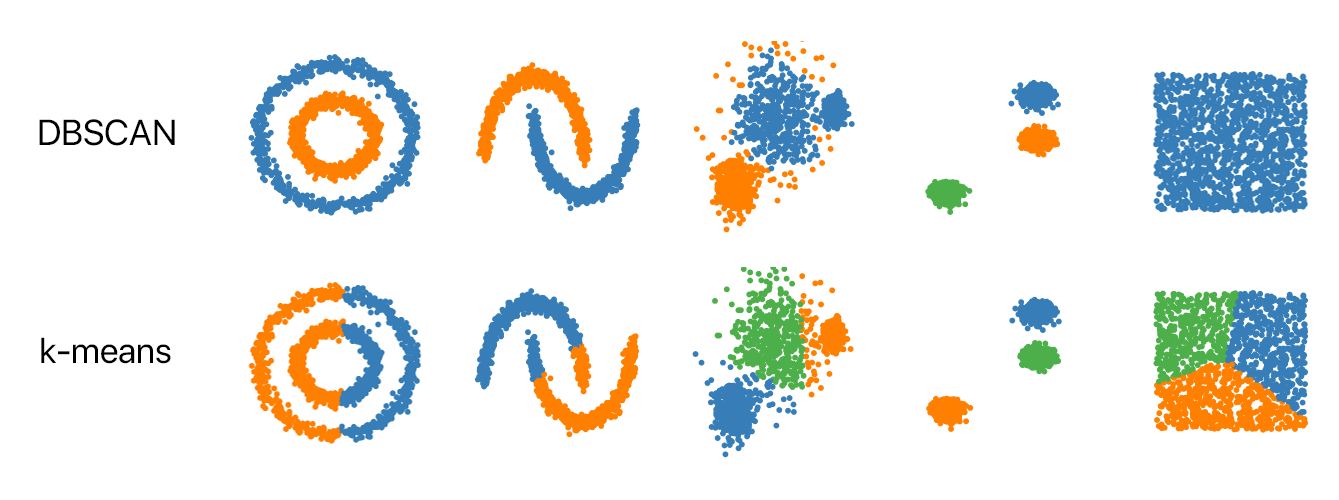
\includegraphics[width=0.5\textwidth]{images/dbscanVSkmeans.png}
    \captionsetup{width=0.6\textwidth}
    \caption{A comparison showing DBSCAN's ability to identify non-spherical clusters, in contrast to K-Means.}
    %\caption{DBSCAN Clustering Compared to K-Means: DBSCAN can identify clusters of arbitrary shapes and effectively handle noise, while K-Means tends to form spherical clusters and is sensitive to outliers.}
    \label{fig:dbscan_vs_kmeans}
\end{figure}

Key Parameters in DBSCAN:
\begin{itemize}
    \item eps ($\epsilon$): The maximum distance between two samples for one to be considered as in the neighborhood of the other.
    \item MinPts: This is the minimum number of points required within the eps radius to form a dense region. 
\end{itemize}
%1. eps: defines the radius of the neighborhood around a data point. Commonly determined with a k-distance graph Analysis. 
%Choosing the ips is Critical: If eps is too small most points will be classified as noise and if it is too large clusters may merge and the algorithm may fail to distinguish between them.
%2. MinPts: This is the minimum number of points required within the eps radius to form a dense region. 
%For most cases a minimum value of MinPts = 3 is recommended


These characteristics make DBSCAN exceptionally well-suited for analyzing real-world crime pattern.
This approach is validated by recent research: Chen et al. \cite{chen2019exploring} successfully utilized an extension of DBSCAN to detect crime hotspots from historical theft records %, validating its effectiveness in this domain

\subsection{Real-time Risk Assessment Systems}%or relevance to risk prediction
% Current approaches, GPS-based risk scoring, challenges in real-time implementation
Real-time geospatial risk assessment is the practical application of crime hotspot forecasting in operational safety systems.
While traditional approaches rely on static crime databases and predetermined risk zones, the challenge lies in integrating GPS-enabled systems to continuously process  spatial data  to calculate immidiate risk score.
\\This is the evolution from static hotspot analysis systems to active safety systems.







% --- Main Section Title ---



\section{Vocal Signal Processing for Distress Detection}
\label{vocal_processing_theory}
In real world emergencies, vocal cues such as tone, pitch, and specific keywords can provide critical 
insights into a person's state of distress. This section explores the theoretical foundations of vocal signal processing: 
Speech Emotion Recognition (SER) for emotional states detection %for detecting emotional states from audio signals, 
,Automatic Speech Recognition (ASR) for speech transcription% for transcribing spoken words 
and Natural Language Processing (NLP) for intent analysis. %for analyzing the transcribed text for intent and risk assessment.


\subsection{Speech Emotion Recognition (SER)}%emotion recognition from speech
\label{ser}
Speech contains important information beyond the words themselves, such as the speacker's emotion, pitch and tone.
Speech Emotion Recognition (SER) is the field of study focused on automatically identifying the emotional state of a speaker from their voice by analyzing acoustic and prosodic features—such as pitch, tone, and energy—to classify emotions like anger, happiness, or fear.
\\The process begins with feature extraction, a foundational concept, where meaningful data is derived from the raw audio signal, often using preprocessing  tools like \textbf{Librosa} \cite{librosa}.%todo cite it
\\Modern SER systems employ transformer-based architectures like \textbf{Wav2Vec 2.0} \cite{NEURIPS2020_92d1e1ebWav2Vec} 
which is a self-supervised model that demonstrates superior performance through pre-training on diverse audio data followed by task-specific fine-tuning.
\\For instance, research has shown that Wav2Vec 2.0 can reach an accuracy of 79.58\% on the IEMOCAP benchmark\cite{wang2022finetunedwav2vec20hubertbenchmark},% [Wang et al., 2022], %todo here we cite the paper fl okhrin we cite the offical documentation
validating its selection as a robust theoretical foundation for the distress detection module.


\subsection{Automatic Speech Recognition (ASR)}%speech-to-text conversion
\label{asr}

% Purpose: Explain the theory of converting speech into text.
%
% What to write:
% 1. Define Automatic Speech Recognition (ASR) as the first analytical pathway.
% 2. Discuss the state-of-the-art using large-scale, pre-trained Transformer
%    models, introducing Whisper as a prime example of this architecture.
% 3. Explain the specific scientific challenges of ASR for low-resource and
%    code-switched dialects like Tunisian Arabic.
%
% Papers needed for this subsection:
% - Main model theory: "Robust Speech Recognition via Large-Scale Weak Supervision" (whisper.pdf)
% - Specific application context: "Leveraging Data Collection and Unsupervised Learning..." (tunisian_arabic-speech_recognition.pdf)
Automatic Speech Recognition (ASR) is the process of converting spoken language into written text, enabling machines to understand and process human speech.
\\Modern ASR systems leverage large-scale, pre-trained Transformer models that enable robust speech-to-text conversion across diverse languages and accents.
One prominent example is \textbf{Whisper} \cite{pmlr-v139-radford21aWhisper}
%todo not finished+ we need at least one pic
\subsection{Natural Language Processing (NLP) for Intent Analysis}% intent analysis from transcribed speech
\label{sec:nlp_intent}
%todo
% Purpose: Explain the theory of analyzing the transcribed text for meaning and risk.
%
% What to write:
% 1. Define Natural Language Processing (NLP) as the final stage of the pipeline,
%    which analyzes the output of the ASR module .
% 2. Discuss the theory behind Transformer-based language models like BERT for text
%    classification and the specific task of Intent Analysis.
% 3. Introduce TunBERT as a state-of-the-art application of this theory, fine-tuned
%    on culturally specific datasets to understand the nuances of the Tunisian dialect.
%
% Paper needed for this subsection:
% - Dataset and context: "T-HSAB: A Tunisian Hate Speech and Abusive Dataset" (New_Icalp_2019.pdf)

\subsection{Integration of SER, ASR, and NLP for Distress Detection}%or multi-modal vocal analysis nhbbklmt pipeline : max 3 jomlett.
\label{integration_ser_asr_nlp}
%todo this is only a draft
The integration of Speech Emotion Recognition (SER), Automatic Speech Recognition (ASR), and Natural Language Processing (NLP) forms a comprehensive vocal analysis pipeline for distress detection.
This multi-modal approach leverages the strengths of each component to provide a robust assessment of vocal distress signals.
\\The SER module analyzes the emotional tone of the speech, identifying signs of fear or anxiety that may indicate distress.
Sim ultaneously, the ASR module transcribes the spoken words into text, capturing the explicit content of the communication.
Finally, the NLP module processes the transcribed text to extract intent and context, identifying keywords or phrases that suggest an emergency situation.
By combining emotional cues with linguistic analysis, this integrated pipeline enhances the accuracy and reliability of distress detection, ensuring that both the emotional state and the verbal content are considered in the assessment.


\section{Machine Learning for Behavioral Anomaly Detection}
\label{sec:behavioral_theory}
%todo: use the paper: a suvey on ...
\subsection{Unsupervised Profiling of User Routines}
\label{sec:unsupervised_profiling}
\subsection{ Anomaly Scoring as a Measure of Deviation}
\label{sec:anomaly_scoring}
\subsection{Supervised Classification for Incident Prediction}
\label{sec:supervised_classification}


\chapter{Design and implementation}
\label{ch:4eme}
%todo we need an intro here 

%\section{System Architecture and Data management}
\section{System Architecture, Integration, and Decision Engine Overview}
\label{sec:system_architecture}
This section outlines the overall architecture of the multi-modal safety system, detailing the technical stack, data management strategies, and the design of the final decision engine.
\subsection{Overall System Architecture}
This system integrates three AI modules: geospatial analysis, vocal signal processing, and behavioral profiling, into a cohesive framework. 
Each module processes its respective data stream and combined, they form a unified risk assessment platform, as shown in figure \ref{fig:architecture}.
\begin{figure}[h!] % placement options: h=here, t=top, b=bottom, p=page
    \centering
    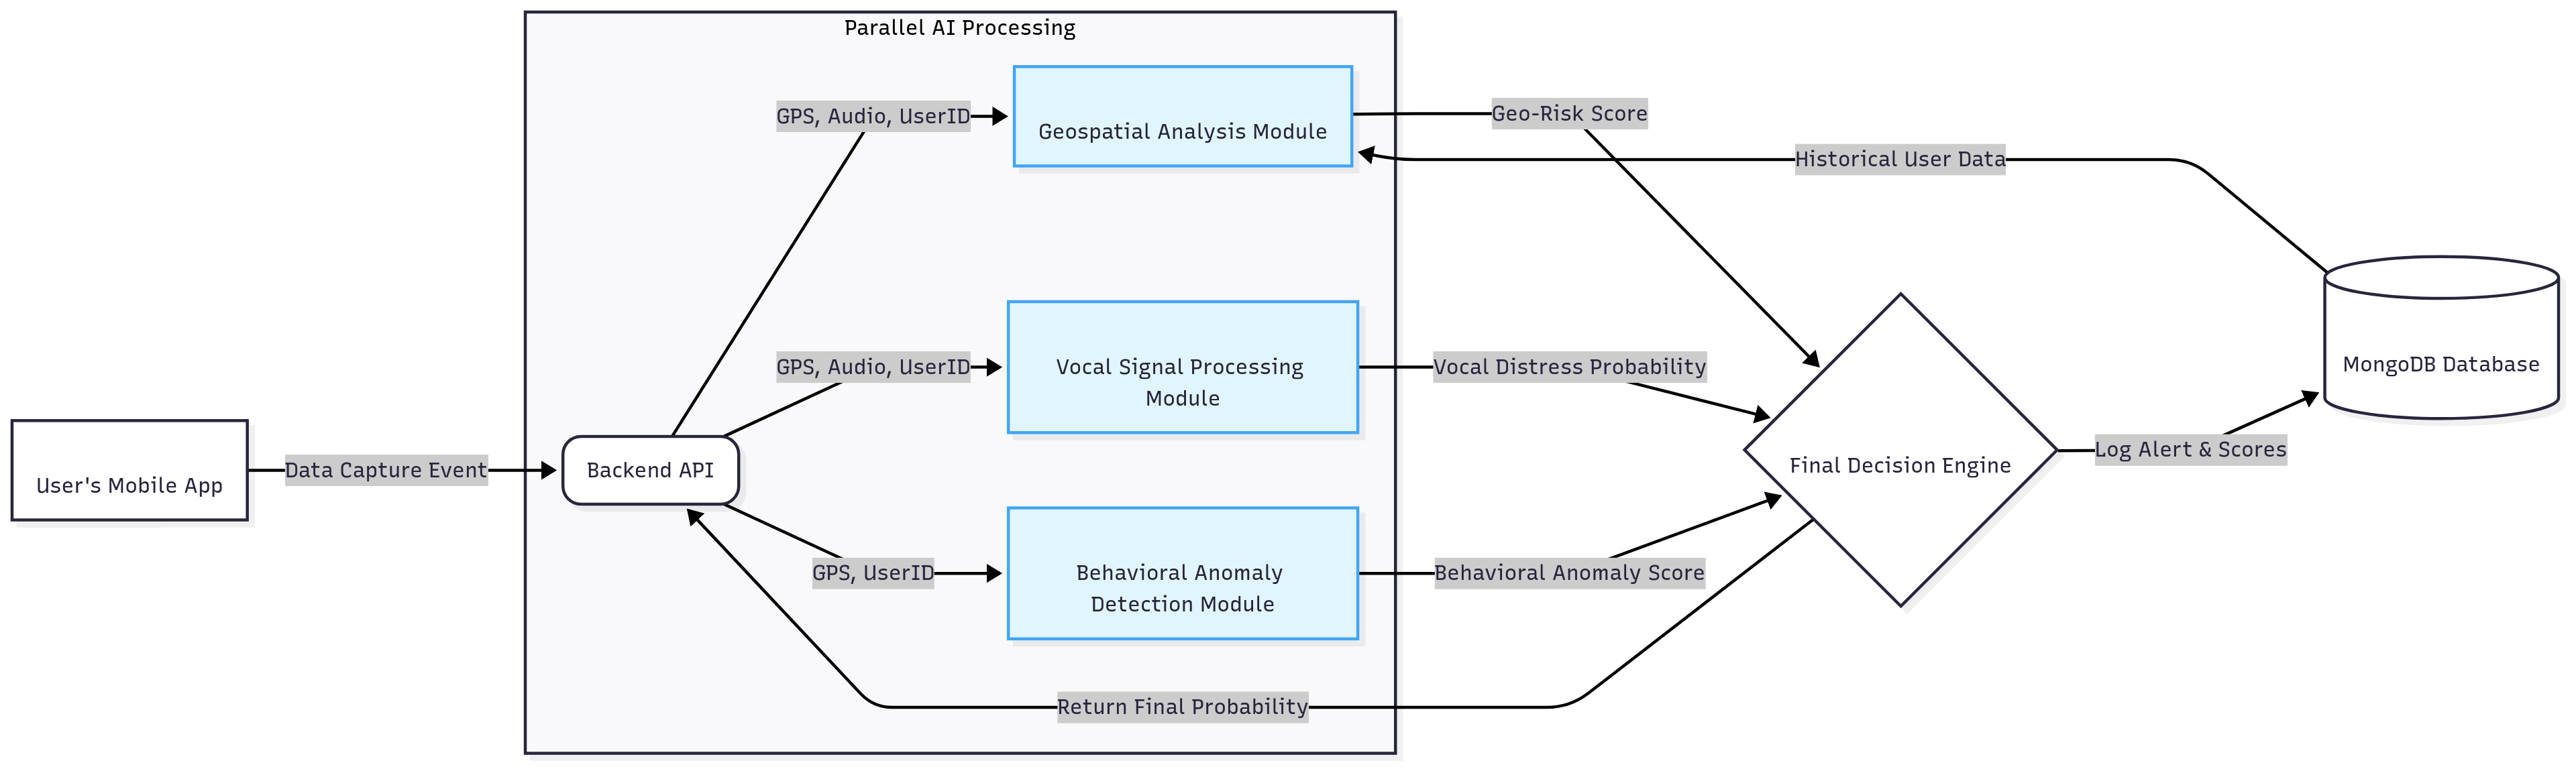
\includegraphics[width=0.9\textwidth]{images/diag5.png}
    \caption{Architecture Diagram of the System}
    \label{fig:architecture}
\end{figure}


\subsection{System Integration and API Design}
\subsection{Technical stack and tools used}
\subsection{Data Management and Preprocessing}
\subsection{Final Decision Engine Design }

\section{Implementation of the Geospatial Analysis Module}
\section{Implementation of the Vocal Signal Processing Pipeline}
\section{Implementation of the Behavioral Profiling Module} % or the Behavioral Anomaly Detection Module or the Machine Learning Module
\section{Final Decision Engine and System Integration}
%this may be merged with the first section (dont know shkoun shyemshi bahtha sahbou ( hawka naamlou referencing lel sections elli will tailor the details if nkaddmou el decision engine kbal les ai modules))

\chapter{Results and Discussion}

\section{Evaluation and Results}
\section{Discussion}








%\section*{Conclusion}
%\section{Conclusion}
\chapter*{Conclusion and perspectives}
\addcontentsline{toc}{chapter}{Conclusion and perspectives}
\markboth{Conclusion and perspectives}{}

\begin{appendix}
\chapter{Appendix 1}
Insert your appendixes here if you need.
\end{appendix}

%\spacing{1}
\bibliographystyle{unsrt}
\bibliography{references}
\end{document}